\chapter*{Konzeptentwurf}
\label{cha:Konzeptentwurf}

\section*{State Machine}
\label{sec:State Machine}

\subsection*{Initialzustand}
\label{subsec:Initialzustand}

Das System startet im Initialzustand und wechselt unmittelbar in den sogenannten Idle-Zustand. Im Idle-Zustand sind beide LEDs der Anzeige AC2398 ausgeschaltet. Von diesem Zustand aus kann es, abhängig von den detektierten Eingaben oder Ereignissen, zu verschiedenen Zustandsübergängen kommen. Wird der grüne Knopf betätigt, während kein RFID-Tag erkannt wird, speichert das System die aktuelle Systemzeit und verbleibt im Idle-Zustand, wie im Diagramm als "Save Time" markiert.

\subsection*{Tag-Erkennung und Verarbeitung}
\label{subsec:Tag-ErkennungundVerarbeitung}

Wird ein NFC-Tag detektiert, wechselt das System in den Zustand "Tag Detected Handling". In diesem Zustand blinkt die grüne LED mit einer Frequenz von einer Sekunde, um die Erkennung des Tags anzuzeigen. In diesem Kontext gibt es zwei mögliche Handlungsoptionen:

Write Tag Handling: Wird der grüne Knopf gedrückt, während das RFID-Tag erkannt wird, erfolgt der Übergang zum Zustand "Write Tag Handling". Hierbei wird die zuvor gesicherte Systemzeit auf das RFID-Tag geschrieben, und die grüne LED leuchtet dauerhaft, um den erfolgreichen Abschluss des Schreibvorgangs anzuzeigen. Sobald das RFID-Tag nicht mehr erkannt wird, kehrt das System in den Idle-Zustand zurück.

Delete Tag Handling: Alternativ kann im "Tag Detected Handling"-Zustand der rote Knopf gedrückt werden, während das RFID-Tag erkannt wird. In diesem Fall erfolgt der Wechsel in den Zustand "Delete Tag Handling". In diesem Zustand werden die gespeicherten Daten des RFID-Tags gelöscht, und beide LEDs leuchten dauerhaft, solange das Tag erkannt wird. Auch hier kehrt das System in den Idle-Zustand zurück, sobald das RFID-Tag nicht mehr erkannt wird.

\subsection*{Fehlerbehandlung}
\label{subsec:Fehlerbehandlung}

Sollte im Verlauf des Prozesses ein Fehler auftreten, wechselt das System in den "Error State Handling"-Zustand. In diesem Zustand blinkt die rote LED mit einer Frequenz von einer Sekunde, während die grüne LED ausgeschaltet bleibt, um den Fehlerzustand zu signalisieren. Der Fehlerzustand bleibt bestehen, bis die Fehlerursache behoben ist. Anschließend erreicht das System den Finalzustand, woraufhin der gesamte Ablauf erneut beginnt.

\begin{figure}[h!]
	\centering
	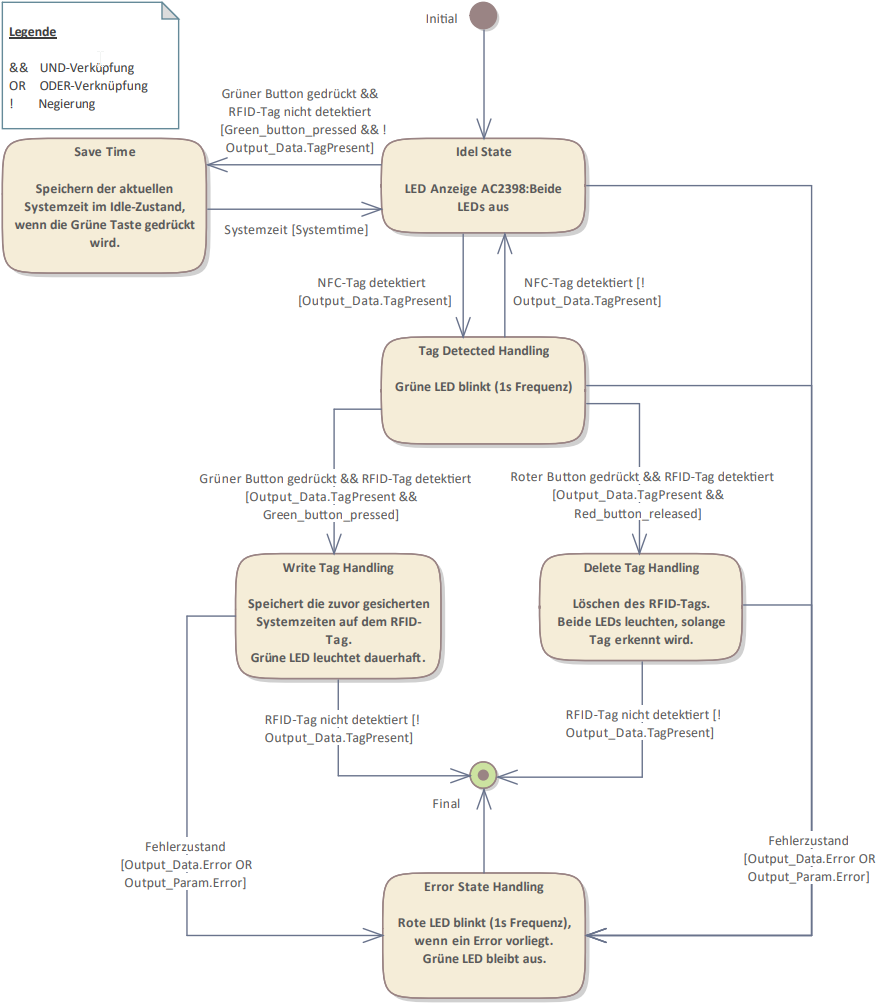
\includegraphics[width=1.0\textwidth]{images/StateMachine.png}
	\caption{State-Machine-Diagramm}
	% [Abbildungsverzeichnis]{Bildunterschrift}
	\label{fig:StateMachineDiagramm}
\end{figure}

\clearpage




\begin{comment} % Aus Angabe:
Erstellung eines Konzept (Planung) mit geeigneter (kompakter) Dokumentation \newline
* Signalliste \\
* Statemachine \\
\end{comment}
Text Text Text...
\begin{table}[h!]
	\centering
	\renewcommand{\arraystretch}{1.0} % Verringert den Zeilenabstand
	\small
	\begin{tabular}{|l|l|l|l|}
		\hline
		\textbf{Name} & \textbf{Datentyp} & \textbf{Adresse} & \textbf{Kommentar}\\ \hline
		RED\_button\_released & Bool & \%I193.2 &  \\ \hline
		Green\_button\_pressed & Bool & \%I193.3 &  \\ \hline
		Red\_button\_LED\_ON & Bool & \%Q192.0 &  \\ \hline
		Green\_button\_LED\_ON & Bool & \%Q192.1 &  \\ \hline
	\end{tabular}
	\caption{Variablentabelle von AC2398}
	\label{tab:AC2398}
\end{table}
\begin{table}[h!]
	\centering
	\renewcommand{\arraystretch}{1.0} % Verringert den Zeilenabstand
	\tiny
	\begin{tabular}{|l|l|l|l|}
		\hline
		\textbf{Name} & \textbf{Datentyp} & \textbf{Adresse} & \textbf{Kommentar} \\ \hline
		Output\_Param.Done & Bool & \%I6.0 & \\ \hline
		Output\_Param.Busy & Bool & \%I6.1 & \\ \hline
		Output\_Param.Error & Bool & \%I6.2 & \\ \hline
		Output\_Param.Status & Word & \%IW8 & \\ \hline
		Output\_Param.ExtStatus & DWord & \%ID10 & \\ \hline
		Output\_Param.RdValue & UInt & \%IW14 & \\ \hline
		Output\_Data.TagPresent & Bool & \%I92.0 & \\ \hline
		Output\_Data.Done & Bool & \%I92.1 & \\ \hline
		Output\_Data.Busy & Bool & \%I92.2 & \\ \hline
		Output\_Data.Error & Bool & \%I92.3 & \\ \hline
		Output\_Data.Status & Word & \%IW94 & \\ \hline
		Output\_Data.ExStatus & Word & \%IW96 & \\ \hline
		Input\_Param.Execute & Bool & \%Q0.0 & \\ \hline
		Input\_Param.Mode & UInt & \%QW2 & \\ \hline
		Input\_Param.SetValue & UInt & \%QW4 & \\ \hline
		Input\_Data.DT\_InAddr & UInt & \%QW16 & \\ \hline
		Input\_Data.DT\_OutAddr & UInt & \%QW18 & \\ \hline
		Input\_Data.Execute & Bool & \%Q20.0 & \\ \hline
		Input\_Data.Force & Bool & \%Q20.1 & \\ \hline
		Input\_Data.Mode & UInt & \%QW22 & \\ \hline
		Input\_Data.TagMemAddr & UInt & \%QW24 & \\ \hline
		Input\_Data.Length & UInt & \%QW26 & \\ \hline
		Input\_Data.WrData & Array[0..31] of UInt & \%Q28.0 & \\ \hline
		Input\_Data.RdData & Array[0..31] of UInt & \%Q60.0 & \\ \hline
	\end{tabular}
	\caption{Variablentabelle von DTI515}
	\label{tab:DTI515}
\end{table}

\clearpage


% ------------------------------------------------------------------------------------
%... Text Konzeptentwurf: Gegenüberstellung verschiedener Lösungsansätze und Lösungsgenerierung, etc.